\documentclass[12pt,a4paper]{article}
\usepackage{fontenc}[T1]
\usepackage{algorithm}
\usepackage{algorithmic}
\usepackage{amsfonts}
\usepackage{amsmath, array}
\usepackage{amsthm}
\usepackage{vmargin}
\usepackage{multicol}
\usepackage{graphicx}
\usepackage{subcaption}
\usepackage{enumerate}
\usepackage{mathtools}
\usepackage{algorithmic}
\usepackage{tikz}
\definecolor{violet}{cmyk}{0.79,0.88,0,0}

\tikzstyle{vertex}=[draw,circle,text=violet,minimum width=20pt]
\setmargrb{19.0mm}{12.0mm}{19.0mm}{12.0mm}%{left}{up}{right}{down}

\DeclarePairedDelimiter\ceil{\lceil}{\rceil}
\DeclarePairedDelimiter\floor{\lfloor}{\rfloor}

\newtheorem{theorem}{Theorem}[section]
\newtheorem{corollary}{Corollary}[theorem]
\newtheorem{lemma}[theorem]{Lemma}
\newtheorem{definition}{Definition}
\newtheorem*{remark}{Remark}
\newcommand{\pa}{\mathtt{a}}
\newcommand{\pb}{\mathtt{b}}

\title{Finding Counterfeit Coin by Pairwise Comparisons}
\author{}

\begin{document}
\maketitle
\documentclass[12pt,a4paper]{article}
\usepackage{algorithm}
\usepackage{algorithmic}
\usepackage{amsfonts}
\usepackage{vmargin}
\setmargrb{19.0mm}{12.0mm}{19.0mm}{12.0mm}%{left}{up}{right}{down}


\begin{document}


Question:
Now we have a's "+" and b's "-", each time we can choose 2 of them to check if they are the same or not.  $\tau(a,b)$ is the minimum number of testing that we can garantee to find a different pair "+" and "-".  \\


Idea:
Consider a graph G(a,b) contains two part, one is $K_a$, another is $K_b$, then we want to find a graph g(a,b) (vetex is not greater than a+b), ang g(a,b) is not a subgraph of G(a,b). Let $t =$ numer of edge of g(a,b), then through  $t$ testing we can   garantee to find a different pair "+" and "-".  \\

Proof:
We tesing as edge of g(a,b). If we can't find the pair "+" and "-" after "t" testing, we can assign a's "+" and b's "-" into g(a,b),  then g(a,b) is the subgraph og G(a,b). By contradiction. \\

Lemma:
 $\tau(a,b)= min(t)$ \\

Proof:
For any graph contains the nunber of edges is less than $min(t)$, imply the graph is a subgraph of G(a,b), then we can conclude that exist a probability greater than 0 that we can not  find a different pair "+" and "-".  \\

Conclusion:
We  want to find a graph g(a,b) that has minimum edges and g(a,b) is not the subgraph of G(a,b), then number of edges of g(a,b) is the answer. \\ 






\end{document}
\section{An Equivalence Graph Problem}


We can present a set of comparisons as a graph. Vertice are the coins, edges are the comparisons.


\begin{definition}
If comparing the edges of a graph results in at least one unbalanced edge in any condition.
We say this graph is a testing solution, feasible. Otherwise it's infeasible.
An optimal testing solution(denoted by $OTS$) is a solution with minimum number of edges(comparisons).
\end{definition}

An $OTS$ can presented by an integer partition as well, which is covered in Section 3.

\subsection*{Idea}
Consider a graph ${\cal G}(\pa,\pb)$ contains two disjoint cliques, one is $K_\pa$, another is $K_\pb$. The edges in ${\cal G}(\pa,\pb)$ means comparing the pair would results in balanced. Then we want to find a graph $g$ (number of vertices $\leq \pa+\pb$) which is not a subgraph of ${\cal G}(\pa,\pb)$.

\begin{lemma}
We can guarantee a graph $g$ (number of vertices $\leq \pa+\pb$) has a unbalanced edge iff $g$ is not a subgraph of ${\cal G}(\pa,\pb)$.
\end{lemma}

\begin{proof}

Denote the real coins as '+' and the fake ones as '$-$'. 

We compare edges of $g$. Vertices of $g$ are subset of vertices of ${\cal G}(\pa,\pb)$.
If $g$ is a subgraph of ${\cal G}(\pa,\pb)$, assign '+'s and '$-$'s from ${\cal G}$ to $g$ , $g$ results in all balance.
If it's not a subgraph of ${\cal G}(\pa,\pb)$, then at least one edge results in unbalance. We can prove this by contradiction. If $g$ results in all balance, edges in $g$ are either ('+','+') or ('$-$','$-$'), subset of edges of ${\cal G}(\pa,\pb)$, thus $g$ is a subgraph of ${\cal G}(\pa,\pb)$.
\end{proof}

\begin{figure}[H]
  \centering
  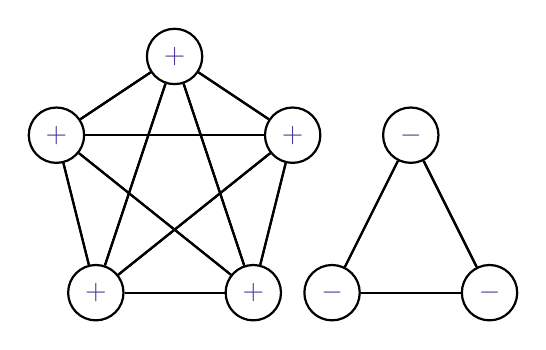
\begin{tikzpicture}[auto, thick]
\tikzstyle{vertex}=[draw,circle,text=violet,minimum width=20pt]
  \foreach \place/\name in {{(0,0)/a},
                            {(-0.5,2)/b},
                            {(2,0)/c},
                            {(2.5,2)/d},
                            {(1,3)/e}}
    \node[vertex] (\name) at \place {$+$};
  \foreach \place/\name in {{(3,0)/f},
                            {(5,0)/g},
                            {(4,2)/h}}
    \node[vertex] (\name) at \place {$-$};
  \foreach \source in {a,b,c,d,e}
    \foreach \dest in {a,b,c,d,e}
      \path (\source) edge (\dest);
  \foreach \source in {f,g,h}
    \foreach \dest in {f,g,h}
      \path (\source) edge (\dest);
\end{tikzpicture}
  \caption{${\cal G}(3,5)$}
\end{figure}

\begin{figure}[!htb]
  \minipage{0.3\textwidth}
    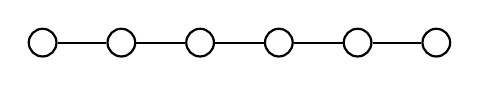
\begin{tikzpicture}[auto, thick]
\tikzstyle{vertex}=[draw,circle,text=violet,minimum width=10pt]
  \foreach \place/\name in {{(0,0)/a},
                            {(1,0)/b},
                            {(2,0)/c},
                            {(3,0)/d},
                            {(4,0)/e},
                            {(5,0)/f}}
    \node[vertex] (\name) at \place {};
  \foreach \source/\dest in {a/b,b/c,c/d,d/e,e/f}
      \path (\source) edge (\dest);
\end{tikzpicture}
    \caption{a trivial solution}
  \endminipage\hfill
  \minipage{0.3\textwidth}
    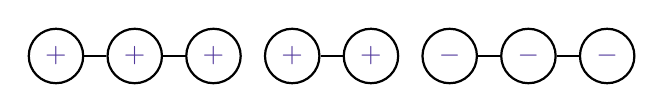
\begin{tikzpicture}[auto, thick]
\tikzstyle{vertex}=[draw,circle,text=violet,minimum width=15pt]
  \foreach \place/\name in {{(0,0)/a},
                            {(1,0)/b},
                            {(2,0)/c},
                            {(3,0)/g},
                            {(4,0)/h}}
    \node[vertex] (\name) at \place {$+$};
  \foreach \place/\name in {{(5,0)/d},
                            {(6,0)/e},
                            {(7,0)/f}}
    \node[vertex] (\name) at \place {$-$};
  \foreach \source/\dest in {a/b,b/c,d/e,e/f,g/h}
      \path (\source) edge (\dest);
\end{tikzpicture}
    \caption{not a solution since it's a subgraph of ${\cal G}(3,5)$, we can assign '+'s and '-'s as in the figure such that all edges are balanced.}
  \endminipage\hfill
  \minipage{0.3\textwidth}
    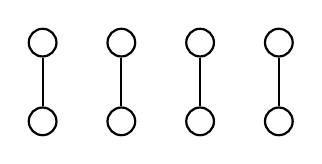
\begin{tikzpicture}[auto, thick]
\tikzstyle{vertex}=[draw,circle,text=violet,minimum width=10pt]
  \foreach \place/\name in {{(0,0)/a},
                            {(0,1)/b},
                            {(1,0)/c},
                            {(1,1)/d},
                            {(2,0)/e},
                            {(2,1)/f},
                            {(3,0)/g},
                            {(3,1)/h}}
    \node[vertex] (\name) at \place {};
  \foreach \source/\dest in {a/b,c/d,e/f,g/h}
      \path (\source) edge (\dest);
\end{tikzpicture}
    \caption{an optimal solution.}
  \endminipage
\end{figure}

Intuitively, if finding unbalance in a comparison, the game ends. But sometimes we can point a pair is unbalance after k comparisons(k is the answer) before the unbalance appears. The following shows $k_{min}=t_{min}-1$, which means the answer for Problem 4 is $t_{min}-1$

\begin{lemma}
$t_{min} = k_{min}+1 $
\end{lemma}

\begin{proof}
We divide the proof of the equation into two inequations

If we could point out a pair $e$ is unbalanced through the optimal graph $F$(with $k_{min}$ comparisons).
Consider a graph with these $k_{min}$ edges + $e$ which is not a subgraph of ${\cal G}(\pa,\pb)$
\[t_{min}\leq k_{min}+1\]

For a optimal graph $E$(with $t_{min}$ edges) which is not a subgraph of ${\cal G}(\pa,\pb)$. Let $E'$ = ($E$ remove an arbitrary edge $e$), then through $E'$. If $E'$ has unbalance comparison, we conclude the one is unbalanced, otherwise we could conclude $e$ is unbalanced.
Either case shows $E'$ is enough to end the game.
\[k_{min} \leq t_{min}-1\]

From the above inequations, the lemma holds.

\end{proof}

\subsection*{Goal}
We want to find a graph $g(\pa,\pb)$ that has minimum edges and $g(\pa,\pb)$ is not a subgraph of ${\cal G}(\pa,\pb)$. Through testing $g(\pa,\pb)-$an arbitrary edge $e$, we can point out a pair is unbalanced and it's optimal.

\begin{definition}
$\tau(\pa,\pb)$ is the number of edges of $OTS(\pa,\pb)$
\end{definition}

For example, $\tau(1,2)=2$, since testing a pair may result in balanced. On the other hand, testing two non-duplicate pair, one of them must results in unbalanced.

In this case, testing a pair is enough to point out a real coin and a fake one. 

Denote the coins we test as $coin_a$ $coin_b$ , the coin we didn't test as $coin_c$
If $coin_a$ and $coin_b$ is not balanced, then point out $coin_a$ and $coin_b$. Otherwise, point out $coin_a$ and $coin_c$

\begin{theorem}
Any graph with $n \leq \pa + \pb$ vertices and $m \leq \lfloor (\pa+\pb)/2 \rfloor-1$ edges $(0<\pa \leq \pb)$ 
is always a subgraph of ${\cal G}(\pa,\pb)$ (or equivalently, a subgraph of ${\cal G}(\pb,\pa)$).
\end{theorem}

\begin{proof}
We shall prove this theorem by induction.  \\

\noindent
{\bf (Basis Case:)} If $\pa = \pb =1$, then $\lfloor (\pa+\pb)/2 \rfloor-1 = 0$. Any graph with $n \leq 2$ vertices and $m \leq 0$ edges (i.e., no edges) is always a subgraph of ${\cal G}(1,1)$.
\\

\noindent
{\bf (Inductive Case:)} Suppose that the theorem holds for all $\pa + \pb \leq k$.  Our target is to show that the theorem also holds for the case $\pa + \pb = k + 1$ with $\pa \leq \pb$.   Consider a graph $G$ with  $n \leq k+1$ vertices and with $m \leq \lfloor (k+1)/2 \rfloor -1$ edges. 

\begin{enumerate}
  \item If $G$ is connected, then $n \leq m + 1 \leq (k+1)/2 \leq b$, which is a subgraph of $K_b$, 
           and thus a subgraph of ${\cal G}(\pa,\pb)$.   

  \item Otherwise, $G$ is not connected.  If $G$ has no edges, then $G$ is obviously a subgraph of ${\cal G}(\pa,\pb,0)$ 
          since $G$ has at most $\pa+\pb$ vertices.
          Else, let $C$ be the connected component of $G$ with the largest number $n'$ of vertices (so that $n' \geq 2$.
          Then, the number of edges in $C$ is at least $n'-1$.  To complete the proof, it is sufficient to show 
          that $G - C$ is a subgraph of ${\cal G}(\pa, \pb - n')$, as we can map $C$ as a subgraph in $K_b$.

The number of vertices in $G-C$ is $k+1-n' = \pa + (\pb-n')$, and the number of edges of $G-C$ is at most 
\begin{eqnarray*}
m - (n'-1) \leq \floor{(k+1)/2} - n' &=& \floor{(k+1)/2 - n'} \\
&=& \floor{ (k+1-n')/2 - n'/2 } \\
&\leq& \floor{ (k+1-n')/2 - 1 } \\
&=& \floor{(k+1-n')/2} - 1 = \floor{ (\pa + (\pb+n'))/2 } - 1.
\end{eqnarray*}
By induction hypothesis, $G-C$ is a subgraph of ${\cal G}(\pa, \pb-n')$, 
and consequently $G$ is a subgraph of ${\cal G}(\pa,\pb)$.
\end{enumerate}
In all cases, $G$ is a subgraph of ${\cal G}(\pa,\pb)$.  This completes the proof of the induction case, so that by the principle of mathematical induction, the theorem follows.
\end{proof}

\begin{corollary}
for all odd number $\pa,\pb$, $\tau(a,b)=\frac{\pa+\pb}{2}$
\end{corollary}

Consider a graph  $g(a,b)$ that have  $\frac{a+b}{2}$ components, each components have only two nodes. then  $g(\pa,\pb)$ is not a subgraph of  ${\cal G}(\pa,\pb)$, and by Thm2.2, it is the optimal solution.

\begin{theorem} 
For every $a,b$, we have a 2-approximation solution of  $\tau(\pa,\pb)$.
\end{theorem}
Consider a line with $max(\pa,\pb)$ nodes as in Figure 2. The graph is not a subgraph of  ${\cal G}(\pa,\pb)$, and by Thm2.2, it is a 2-approximation solution.

\section{Integer Partition}

\noindent
To find $g(\pa,\pb)$ with minimal number of edges, it's obvious that $g(\pa ,\pb)$ should not form a cycle

\begin{proof} 
if $g(\pa,\pb)$ form a cycle, remove an edge, the number of vertices each component remains same, whether $g'(\pa,\pb)$ is the subgraph of ${\cal G}(\pa,\pb)$ is equivalent to whether $g(\pa,\pb)$ is the subgraph of ${\cal G}(\pa,\pb)$
\end{proof}

\begin{definition}
We define a multiset avoids $x$ iff its subset-sums has no $x$, a partition avoids $x$ iff its parts avoids $x$
\end{definition}

\begin{theorem}

the problem would be transformed to find a partition of $\pa+\pb$ with  maximal number of parts that avoids $\pa$

\end{theorem}

\begin{proof} 
Let $t =$ number of edge of $g(\pa,\pb)$

$n$ as number of componets in $g(\pa,\pb)$

$M$ as the set of components

% $m$ as the set of number of vertices

% $m_i$  as number of vertices of $i$th component

since $g(a,b)$ doesn't contain any cycle, $t = \pa+\pb - n$, to find minimal t is equivalent to find maximal n such that $g(\pa,\pb)$ is not the subgraph of ${\cal G}(\pa,\pb)$

if $g(\pa,\pb)$ is the subgraph of ${\cal G}(\pa,\pb)$, 
since each component is conected, each one is either in $K_a$ or $K_b$, there exist a subset of M in $K_a$ the number of vertices of M = a
,e.g there exist a subset of m is equal to $a$

if $g(\pa,\pb)$ is not the subgraph ${\cal G}(\pa,\pb)$, there must not a subset of m is equal to $a$, since if there subset of m is equal to $a$ let these componets in $K_a$ and others in $K_b$, then $g(\pa,\pb)$ is the subgraph ${\cal G}(\pa,\pb)$ thus raise contradiction


the sum of $m$ is $\pa+\pb$, so the theorem holds

\end{proof}

\begin{definition}
$\rho(\pa,\pb)$ is the maximal number of parts of $\pa+\pb$ avoids $\pa$

$d$ is the smallest non-factor of $\pa$
\end{definition}

\begin{remark}
$\tau(\pa,\pb)=\pa+\pb-\rho(\pa,\pb)$
\end{remark}

\begin{theorem}
Optimal partition for $\pa=2$

\[
 \rho(2,\pb) =
   \begin{cases}
     1+\frac{\pb}{3}   &\mbox{if }\pb\equiv0\\
     1+\frac{\pb-1}{3} &\mbox{if }\pb\equiv1\\
     1+\frac{\pb+1}{3} &\mbox{if }\pb\equiv2
   \end{cases}
   \pmod{3}
\]
\end{theorem}

\begin{proof}
	since there is no $a$ in subset sums of the partition $P$, there is at most one '$1$' and no '$2$' in $P$, $|P|\leq \floor{\frac{\pb+2}{3}}$

	for $\pb\equiv0\pmod{3}$, there exist an optimal partition $P=\{1,4,3,...\}$('...' are '$3$'s) that reaches optimal bound and avoids $\pa$

	for $\pb\equiv1\pmod{3}$, there exist an optimal partition $P=\{1,5,3,...\}$('...' are '$3$'s) that reaches optimal bound and avoids $\pa$

	for $\pb\equiv2\pmod{3}$, there exist an optimal partition $P=\{1,3,3,...\}$('...' are '$3$'s) that reaches optimal bound and avoids $\pa$

\end{proof}


\subsection{Exact Algorithm}

\begin{algorithmic}
  \STATE{$R= \{\pa+\pb\}$}
  \FOR{\textbf{each} partition $P$ of the number $\pa+\pb$ which avoids $\pa$}
    \IF{$|P|>|R|$} \STATE{$R=P$}
    \ENDIF
  \ENDFOR
  \STATE{output $R$}
\end{algorithmic}
check P's avoidence by Dynamic-Programming as solving discrete knapsack problem, keep avoidence vector when enumerating.

Denote the number of partitions of $n$ as $p(n)$

Denote the number of partitions avoids $a$ of $n$ as $p_{aoivds\ a}(n)$

Time Complexity: 

\[
O(a\times p_{aoivds\ \pa}(\pa+\pb))\\
\leq O(\pa\times p(\pa+\pb))\\
\leq O(\pa\frac{exp(\sqrt{\frac{2(\pa+\pb))}{3} } )}{\pa+\pb})
\]

\pagebreak
\subsection{Results}
\input{rhotauTable.tex}
\pagebreak
%!TEX root = total.tex

\section{Finding Optimal Foolproof Scheme}
Based on Corollary~\ref{cor:maximize-|P|} in the previous section, we can find an optimal foolproof scheme 
by enumerating all possible partitions of $\pa+\pb$, and selecting among those that avoids $\pa$ the one 
that consists of the most number of parts.  This approach is equivalent to solving the NP-complete 
{\sc Subset Sum} problem~\cite{GarJoh79} for each possible partition of $\pa+\pb$, 
which can be done via dynamic programming~\cite{CLRS09} as shown in Algorithm~\ref{algo:naive}:

\begin{algorithm}
\caption{Find Optimal Foolproof Scheme (OFS)}
\label{algo:naive}
\begin{algorithmic}
  \Procedure{Find\_Optimal\_Foolproof\_Scheme}{$\pa,\pb$}\Comment{Return an OFS}
    \State{Set default partition $R$ as $\{\pa+\pb\}$;}
    \For{\textbf{each} partition $P$ of the number $\pa+\pb$ which avoids $\pa$}
      \If{Subset\_Sum($P,\pa$)} \State \bf continue
      \ElsIf{$|P|>|R|$} \State{update $R$ as $P$;}
      \EndIf
    \EndFor
    \State{\textbf{return} $R$}
  \EndProcedure
  \end{algorithmic}
\begin{algorithmic}
  \Procedure{Subset\_Sum}{$P,\pa$}\Comment{Check if a subset of $P$ sums up to $\pa$}
    \State Set default multiset $S$ as $\{0\}$;
    \For{\textbf{each} integer $\pi \in P$} 
      \State{$S \leftarrow S \cup \{\pi + s \mid s \in S \mbox{\ and\ } \pi + s \leq \pa \}$;}
    \EndFor
    \State \textbf{return} $a \in S$
  \EndProcedure
\end{algorithmic}
\end{algorithm}

Let $p(n)$ denote the number of different partitions of $n$, 
which asymptotically approaches $\smash{\mathrm{exp}(\pi\sqrt{2n/3})/(4n\sqrt{3})}$ 
as $n \rightarrow \infty$~\cite{HarRam18}.   
The running time of the procedure Subset\_Sum$(P,\pa)$
is $|P| \times O(\pa)$, which is bounded by $O((\pa + \pb)\pa)$.  Thus, by Algorithm~\ref{algo:naive}, 
we can find an optimal foolproof scheme, as well as compute the value of $\tau(\pa,\pb)$, in 
$$p(\pa+\pb) \times O((\pa+\pb)\pa) = O\left(\pa \ e^{\pi\sqrt{2(\pa+\pb)/3}}\right) \mbox{\ time.}$$  
\ref{sec:results} shows a table of $\tau(\pa,\pb)$ for $1 \leq \pa, \pb \leq 15$.

\medskip

\noindent
{\it Remark.} If we enumerate the partitions by depth-first search (according to lexicographical order), 
                      consecutive partitions during the enumeration will generally be similar, so that 
                      the time for Subset\_Sum$(P,\pa)$ for each partition requires amortized $O(\pa)$ time.
                     Consequently, this allows us to reduce the time complexity further by a factor of $O(\pa+\pb)$.
                     Nevertheless, this is not the main focus of the work, so that we omit the details for brevity.

\subsection{Cyclic Property of $\tau(\pa,\pb)$}
In this subsection, we shall show that for any $\pa$, 
there is some property that an optimal foolproof scheme must possess when $\pb$ is sufficiently large.
Consequently, this allows us to show a cyclic property about $\tau(\pa,\pb)$, 
as well as speed up the construction time of an optimal foolproof scheme. 

\medskip

\noindent
Before delving into details, let us take a look about the values $\tau(2,\pb)$ and $\tau(5,\pb)$ for different $\pb$s.

\medskip

\begin{tabular}{c|rrrrrrrrrrrrrrr}
$\pb$ &  1 &  2 &  3 &  4 &  5 &  6 &  7 &  8 &  9 & 10 & 11 & 12 & 13 & 14 & 15  \\
\hline
$\tau(2,\pb)$  &  2 &  2 &  3 &  4 &  4 &  5 &  6 &  6 &  7 &  8 &  8 &  9 & 10 & 10 & 11 \\
$\tau(5,\pb)$        &  3 &  4 &  4 &  5 &  5 &  6 &  6 &  8 &  7 & 10 &  8 & 11 &  9 & 12 & 10  \\
\hline
\end{tabular}

\medskip

\noindent
From $\pb\geq 1$, $\tau(2,\pb)$ forms cycle of length $3$, such that $\tau(2,\pb+3) = \tau(2,\pb) + 2$.
Similarly, from $\pb\geq 9$, $\tau(5,\pb)$ forms cycle of length $2$, such that $\tau(5,\pb+2) = \tau(5,\pb) + 1$.
In fact, for any fixed $\pa$, such kind of cycles must eventually occur.  
To see why this is true, we shall now examine more closely about the structure of an optimal foolproof scheme.  

\medskip

\noindent
Let $\ell(n)$ denote the least non-factor of $n$, which is the smallest positive integer that does not divide $n$ properly.
For instance, $\ell(1) = 2$, $\ell(2) = 3$, $\ell(3) = 2$, $\ell(4) = 3$, $\ell(5) = 2$, and $\ell(6) = 4$.  
To simplify our discussion, we shall now assume $\pa \leq \pb$ throughout this subsection, and use $\pl$ to denote $\ell(\pa)$.
Also, we call a partition $P$ of $n$ a \emph{maximal} partition that avoids $x$, if among all partitions of $n$ 
which avoid $x$, $P$ is one that contains the maximum number of parts;  furthermore, we use $\rho(x, n)$ to denote its number of parts.
The following two lemmas give some basic properties about a partition that avoids $\pa$.

\begin{lemma} \label{lem:at-least-b/L}
Let $P$ be a maximal partition of $\pa + \pb$ that avoids $\pa$.  
Then, $|P| = \rho(\pa, \pa+\pb) \geq \myceil{\pb/\pl}$.
\end{lemma} 
\begin{proof}
Consider a partition of $\pa+\pb$ with $\myceil{\pb/\pl}-1$ instances of $\pl$ and a remainder part $r = \pa+\pb-\pl(\myceil{\pb/\pl}-1)$.  
For any subset $P'$ of this partition, either $P'$ contains $r$, or $P'$ contains purely copies of $\pl$.  
In the former case, the subset sum of $P'$ cannot be $\pa$, since $r > \pa$. 
In the latter case, the subset sum of $P'$ cannot be $\pa$, since $\pl$ does not divide $\pa$.
Thus, the above partition avoids $\pa$, and contains $\myceil{\pb/\pl}$ parts.   
This completes the proof of the lemma.
\qed
\end{proof}

\begin{lemma} \label{lem:at-most-a-1}
If a partition $P$ avoids $\pa$, $P$ contains less than $\pa$ integers that is a factor of $\pa$;  
in other words, $| \{ \pi \mid \pi \in P \mbox{\ and\ } \pi < \pl \}|  < \pa$. 
\end{lemma}
\begin{proof}
Let $P = \{ \pi_1, \pi_2, \ldots \}$ with $\pi_i \leq \pi_j$ when $i < j$.  
Moreover, let $k$ be the number of integers in $P$ that is a factor of $\pa$
(i.e., $k$ is the largest index such that $\pi_k < \pl$).   

\medskip

\noindent
Let $S_i$ denote the set of integers in $[1,\pa]$ that can be written as a sum from a subset of
integers in $P_i = \{ \pi_1, \pi_2, \ldots, \pi_i \}$.   Thus, if $\pi_1 < \pl$,
we have $S_1 = \{ \pi_1 \}$, and $|S_1| = 1$.
We claim that $|S_i| < |S_{i+1}|$ for any $i \in [1,k-1]$, so that $|S_k| \geq k$.  
Furthermore, since $P$ avoids $\pa$, we must have $|S_k| < \pa$, so that we obtain
the desired relationship that $k < \pa$.

\medskip

\noindent
It remains to prove the claim.  Suppose on the contrary that $|S_i| = |S_{i+1}|$ for some $i \in [1,k-1]$.  
This implies that $\pi_{i+1} \in S_i$, or else $S_{i+1}$ contains at least one more integer than $S_i$.
As $\pi_{i+1} \in S_i$, we must now have $2\cdot \pi_{i+1} \in S_i$ for the same reason.
Inductively, for each $t \geq 1$ such that $t\cdot \pi_{i+1} \leq \pa$, we must have $t\cdot \pi_{i+1} \in S_i$.
Since $\pi_{i+1}$ is a factor of $\pa$, this implies that $\pa \in S_i$.  In other words, $\pa$
can be written as a sum of a subset of integers in $P_i \subseteq P$; this contradicts with the fact that
$P$ avoids $\pa$.  Thus, the claim (and the lemma) follows.
\qed
\end{proof}

Based on the above lemmas, we are ready to establish 
the key lemma and the main theorem of this subsection as follows.

\begin{lemma}  \label{lem:key-lemma}
Let $P$ be a maximal partition of $\pa + \pb$ that avoids $\pa$.
If $\pb > \pl\left((\pl+1)(\pa - 1) + \myceil{\pa/\pl}\right)$,
$P$ must contain at least $\myceil{\pa/\pl} = \myfloor{\pa/\pl} + 1$ instances of $\pl$.
\end{lemma}
\begin{proof} 
We shall prove this by contradiction.  Let us fix a maximal partition~$P$, and use $X_i$ to denote
the number of instances of $i$ contained in $P$.  
Assume on the contrary that $X_\pl \leq \myfloor{\pa/\pl}$.  Then, we have
\[
  |P| = \sum_{1\leq i < \pl}{X_i} + X_\pl +\sum_{i \geq \pl+1}{X_i}.
\]
Since $\sum_i {i \cdot X_i} = \pa+\pb$, under the conditions that  
$\sum_{1\leq i < \pl}{X_i} \leq \pa-1$ by Lemma~\ref{lem:at-most-a-1} and 
$X_\pl \leq \myfloor{\pa/\pl}$ by the assumption, we get
\begin{eqnarray*}
  |P|\ &\leq& \  
       \pa - 1 + \myfloor{\frac{\pa}{\pl}}   +  \frac{(\pa + \pb) - 1 \cdot (\pa-1) - \pl \cdot (\myfloor{\pa/\pl})}{\pl+1}\\
       &=& \  \pa - 1 + \frac{\pb  + 1 + \myfloor{\pa/\pl}}{\pl+1}\ \ =\ \ \pa - 1 + \frac{\pb + \myceil{\pa/\pl}}{\pl+1}.
\end{eqnarray*}  
By Lemma~\ref{lem:at-least-b/L}, we have $|P| \geq \myceil{\pb/\pl} \geq \pb/\pl$, so that
\[
  \frac{\pb}{\pl}\ \ \leq\ \ \pa - 1 + \frac{\pb + \myceil{\pa/\pl}}{\pl+1}.
\]
Multiplying both sides by $\pl(\pl+1)$, we obtain
\[
  \pb(\pl+1)\ \ \leq\ \ \pl(\pl+1)(\pa - 1) + \pb\pl + \pl\myceil{\pa/\pl}.
\]
This contradicts with the condition that $\pb > \pl \left((\pl+1)(\pa-1) + \myceil{\pa/\pl}\right)$, 
and the lemma thus follows.
\qed
\end{proof}

\begin{theorem} \label{thm:OFS-of-P+L}
Let $P$ be a maximal partition of $\pa + \pb$ that avoids $\pa$.
If $\pb > \pl\left((\pl+1)(\pa - 1) + \myceil{\pa/\pl}\right)$, then
$P' = P \cup \{ \pl \}$ must be a maximal partition of $\pa + \pb + \pl$ that avoids $\pa$.
\end{theorem}
\begin{proof}
We first show that $P'$ avoids $\pa$, and then further show that $P'$ is a maximal partition.
Both facts together will complete the proof.

\medskip

\noindent
{\bf $P'$ avoids $\pa$:}  Suppose on the contrary that some subset of $P'$ adds up to $\pa$.  This happens only if some subset of $P$
adds up to $\pa$ or $\pa - \pl$.  The former case cannot occur since $P$ avoids $\pa$.  For the latter case, let $S$ be a subset of $P$ 
whose sum is exactly $\pa - \pl$.  Then, $S$ contains at most $\myceil{\pa/\pl} - 1$ instances of $\pl$ (otherwise the sum exceeds $\pa - \pl$);  
however, by Lemma~\ref{lem:key-lemma}, $P$ contains at least $\myceil{\pa/\pl}$ copies of $\pl$, so that $\pl \in P\backslash S$.
Consequently, $S \cup \{\pl\} \subseteq P$, whose sum is exactly $\pa$.  This contradicts with the assumption that $P$ avoids $\pa$.

\medskip

\noindent
{\bf $P'$ is maximal:}  Suppose on the contrary that there exists some partition $S'$ of $\pa+\pb+\pl$ that avoids $\pa$, and with $|S'| > |P'|$.
By Lemma~\ref{lem:key-lemma}, $S'$ contains at least one instance of $\pl$.  Removing one instance of $\pl$ from $S'$ would give a 
partition $S$ of $\pa + \pb$ that avoids $\pa$, and with $|S| = |S'| - 1 > |P'| - 1 = |P|$.  This contradicts with the maximality of $P$.
\qed
\end{proof}

The above theorem, together with Corollary~\ref{cor:maximize-|P|}, immediately leads to the following corollary:

\begin{corollary}
For sufficiently large $\pb$,  
\begin{eqnarray*}
  \rho(\pa, \pa + \pb + \pl) &=& \rho(\pa + \pb) + 1 \\
  \tau(\pa,\pb+\pl)             &=& \tau(\pa,\pb) + \pl - 1.
\end{eqnarray*}
\end{corollary}

\subsection{Speed-Up in Finding Optimal Foolproof Scheme}
Based on Theorem~\ref{thm:OFS-of-P+L}, we can find an optimal foolproof scheme in an alternative way, as shown in Algorithm~\ref{algo:faster}.  
Basically, if $\pb$ is sufficiently large, we will first calculate a maximum $k$ such that $\pb - k\pl$ remains sufficiently large, 
and construct a maximal partition $P$ of $\pa + \pb - k\pl$ that avoids $\pa$. 
Then, we extend $P$ to a maximal partition $P'$ of $\pa + \pb$ by adding $k$ copies of $\pl$.  Else, we will simply run Algorithm~\ref{algo:naive}
to obtain the answer.  Consequently, for any value of $\pb$, the running time of the algorithm is bounded by 
$$p(\pa + \pl((\pl+1)(\pa-1) + \myceil{\pa/\pl})) \times O(\pa) \approx O\left(e^{\pi\pl\sqrt{2\pa/3}}\right),$$  
which is independent of $\pb$.

\begin{algorithm}
\caption{A Faster Algorithm to Find Optimal Foolproof Scheme}\label{algo:faster}
\begin{algorithmic}
  \Procedure{Faster\_Optimal\_Foolproof\_Scheme}{$\pa,\pb$}\Comment{Return an OFS}
    \If {$\pb > \pl((\pl+1)(\pa-1) + \myceil{\pa/\pl})$}\Comment{$\pl$ is the least non-factor of $\pa$}
        \State {$k \leftarrow$ maximum integer such that $\pb - k\pl > \pl((\pl+1)(\pa-1) + \myceil{\pa/\pl})$;}
        \State {$R\ \leftarrow\ $ Find\_Optimal\_Foolproof\_Scheme$(\pa,\pb - k\pl)$; }         
        \State {\textbf{return} $R \cup \{ \pl, \ldots, \pl \}$; }\Comment{$\{ \pl, \ldots, \pl \}$ = $k$ copies of $\pl$}
    \Else
         \State {\textbf{return} Find\_Optimal\_Foolproof\_Scheme$(\pa,\pb)$;}
    \EndIf
  \EndProcedure
\end{algorithmic}
\end{algorithm}


\section{extended problem}
We shall discuss several problems simular to the foolproof problem in section 1. These are called inference problems. For convenience, we assume fake coins are minor in the whole coins.(e.g. ($\pa\leq \pb $)
In the same way in Section 2, we present a scheme as a graph. There are four inference problems: infering a fake coin,a real coin, real-fake pair, a fake coin and a real coin. We $-$, $+$, $\pm$, $+-$ superscription to denote them seperately.

\subsection*{Infering a real-fake pair}
{
\setlength{\leftskip}{1cm}
\setlength{\rightskip}{1cm}
There are $\pa$ fake coins and $\pb$ real coins ($\pa, \pb > 0$). The real coins are all the same weight and also the counterfeit coins, but two  types are different weight. Each time we compare only two coins have the same weight or not. In this case, assume $\pa$, $\pb$ are known.
Find the smallest number of comparison that we can infer a pair is real-fake. In this problem, we don't need to know which one is fake.\\

}
\begin{definition}
If a scheme could infer a real-fake coin. We say this graph is a inferable$^\pm$ scheme for fake ($\IS^\pm$). Otherwise it's not inferable$^\pm$.

Optimal inferable scheme for fake ($\OIS^\pm$) is $\IS^\pm$ with minimum number of comparison.
Deonte the number of edges of $\OIS^\pm$ by $\tau^\pm(\pa,\pb)$.
\end{definition}

Note that in the foolproof problem. We can infer the pair on the scale which is unbalanced. But sometimes before the unbalance appears, we can infer a pair is real-fake. The following shows the answer is $\tau(\pa,\pb)-1$.

\begin{lemma}
$\OIS^\pm= \text{removing an arbitrary edge}$. That is, $\tau^\pm(a,b)=\tau(a,b)-1$
\end{lemma}

\begin{proof}
We divide the proof of the equation into two inequations. For conciseness, we denote $\tau(a,b)-1$ by $\tau$ and the answer of this problem as $\tau^\pm$.

For a optimal foolproof scheme $G$(with $\tau$ edges). Let $G'$ = ($G$ remove an arbitrary edge $e$), then through $F'$.
If $G'$ has unbalance comparison, we conclude the one is unbalanced, otherwise we could conclude $e$ is unbalanced.
Either case shows $G'$ is sufficient to infer a real-fake pair.
\[\tau^\pm \leq \tau-1\]

If we could infer a pair $e$ is real-fake through the optimal scheme $F$(with $\tau^\pm$ comparisons).
Then the graph $F$ + $e$ is foolproof.
\[\tau\leq \tau^\pm+1\]

From the above inequations, the lemma holds.

\end{proof}
\subsection*{Two conditions of a testing scheme}

When testing a testing scheme, there are two conditions.

\textbf{Condition 1.} there is an unbalanced edges

\textbf{Condition 2.} they are all balanced

For infering a $\pm$, we must ganrantee both conditions work. For Condition 1, we would simplily infer the unbalanced edges. For Condition 2, we would infer the edge must be unbalanced because adding this edge would form a foolproof scheme.
For the following inference problems($-$,$+$,$+-$), we shall use the same logic. 

\subsection*{Infering a fake coin}
{
\setlength{\leftskip}{1cm}
\setlength{\rightskip}{1cm}
\noindent 
There are $\pa$ fake coins and $\pb$ real coins ($\pa, \pb > 0$). The real coins are all the same weight and also the counterfeit coins, but two  types are different weight. Each time we compare only two coins have the same weight or not. In this case, assume $\pa$, $\pb$ are known.
Find the smallest number of comparison that we can infer a coin is fake.\\

}

\begin{definition}
If a scheme could infer a fake coin. We say this graph is a inferable$^-$ scheme for fake ($\IS^-$). Otherwise it's not inferable$^-$.

Optimal inferable scheme for fake ($\OIS^-$) is $\IS^-$ with minimum number of comparison.
Deonte the number of edges of $\OIS^-$ by $\tau^-(\pa,\pb)$.
\end{definition}

Note that $\OFS(a,b)$ could find a real and a fake coin. Thus $\tau(\pa,\pb)$ is an upper bound of $\tau^-(\pa,\pb)$.
A $\IS^-(\pa,\pb)$ better than $\OFS(\pa,\pb)$ must use another strategy, which is, though all comparisons result in balance we could still infer a `$-$'.\\

Before solving $\IS^-$, we observe how a inferable$^-$ scheme works.

For a testing scheme, there are two conditions

If \textbf{Condition 1.} happens then we immediate infer the fake coin from the unbalanced.
If \textbf{Condition 2.} happens, we must claim a fake coin, and this coin couldn't be a real one in any condition, otherwise this inference is wrong.\\

We present an optimal inferable$^-$ scheme as a integer partition for an example. Let (a,b)=(2,6), 
this scheme is [3,3,`1',1] .If \textbf{Condition 2}, we infer the `1' is the fake coin. To explain more, we introduce the following lemma.

\begin{lemma}\label{lma:inferable}
If \textbf{Condition 2}, the scheme is inferable for a fake coin $c_1$ if and only if removing $c_1$'s part, the remaining parts avoids $\pa$. Physically, $c_1$ must not be a real coin with \textbf{Condition 2}.
\end{lemma}

To find a inferable$^-$ better than $\OFS$ must solve \textbf{Condition 2}.
Denote the part of the fake coin to be infered as $i(i\leq\pa)$. 
Beyound the remainning $\pa+\pb-i$ parts, 
(1)they must avoid $\pa$, since if there's a subset sum $\pa$, assign the subset `$+$', this claim is wrong
(2)they must contain $\pa-i$ or equivalently contain $\pb$, since there must exist a condition such that the coin is fake and \textbf{Condition 2}.


\begin{definition}
Same as previous problem, we define $\IS^-$, $\OIS^-$ and $\tau^-(a,b)$.
\end{definition}

Note that $Q(n,a,b)\geq\tau(a,n-a)$\\

For \textbf{Condition 2.}, $1\leq i\leq\pa$ for $\IS^-$, thus we get the following lemma.

\begin{lemma}
$\tau^-(\pa,\pb)=min\{\tau(\pa,\pb), \{i-1+Q(\pa+\pb-i,\pa,\pb) | 1\leq i\leq\pa\} \}$
\end{lemma}

We are ready to solve $\OIS^-$ now.

\begin{theorem}
$\OIS^-(\pa,\pb)=optimal\{\OFS(a,b), \{\text{a tree of i-1 nodes and }\OFS(a,b-i) |1\leq i\leq a\}\}$

$\tau^-(\pa,\pb)=min\{\tau(\pa,\pb), \{i-1+\tau(\pa,\pb-i) | 1\leq i\leq\pa\} \}$
\end{theorem}

\begin{proof}
We divide the proof into inferable$^-$ part and optimal part.

\noindent{\bf (inferable$^-$ Part:)}

For $OFS(a,b)$ could infer a fake coin because only \textbf{Condition 1.} happens.
For $\{\text{a tree of i nodes and }OFS(a,b-i) |1\leq i\leq a\}\}$, if \textbf{Condition 2.}, we infer one coin of the i-node tree as fake coin.

\noindent{\bf (Optimal Part:)}
from lemma 5.2
\begin{align*}
\tau^-(a,b)&=min\{\tau(a,b),\{i-1+Q(a+b-i,a,b) | 1\leq i\leq a\} \}\\
&\geq min\{\tau(a,b), \{i-1+\tau(a,b-i) | 1\leq i\leq a\} \}
\end{align*}

is a optimal lower bound.

And $optimal\{OFS(a,b), \{\text{a tree of i nodes and }OFS(a,b-i) |1\leq i\leq a\}\}$ reaches this lower bound.

\end{proof}

\subsection*{Infering a real coin}

{
\setlength{\leftskip}{1cm}
\setlength{\rightskip}{1cm}
\noindent 
There are $\pa$ fake coins and $\pb$ real coins ($\pa, \pb > 0$). The real coins are all the same weight and also the counterfeit coins, but two  types are different weight. Each time we compare only two coins have the same weight or not. In this case, assume $\pa$, $\pb$ are known.
Find the smallest number of comparison that we can infer a coin is real.\\

}

\begin{definition}
Same as previous problem, we define $\IS^+$, $\OIS^+$ and $\tau^+(a,b)$.
\end{definition}

$\OIS^+$ is trivial.
That is, comparing $\pa$ coins in a group. 

\begin{theorem}
$\OIS^+(\pa,\pb)=\text{a tree of }\pa+1\text{ nodes}$
\end{theorem}
\begin{proof}
We divide the proof into inferable$^+$ part and optimal part.

\noindent{\bf (Inferable$^+$ Part:)}

we omit this part since it's same as previous theorem.

\noindent{\bf (Optimal Part:)}
\begin{align*}
\tau^+(a,b)&=min\{\tau(a,b), \{i-1+Q(a+b-i,b,a) | 1\leq i\leq b\} \}&\\
&\geq min\{\tau(a,b), \{i-1+\tau(a-i,b) | 1\leq i\leq b\} \} &\text{by Theorem 2.2.}\\
&\geq min\{\floor{\frac{a+b}{2}}, i-1+\frac{a-i+b}{2}\}&\\
&\geq min\{a, a\}=a &
\end{align*}

is a optimal lower bound.

$\text{a tree of }\pa+1\text{ nodes}$ reaches optimal lower bound.
\end{proof}

\subsection*{Infering a real coin and a fake coin}

{
\setlength{\leftskip}{1cm}
\setlength{\rightskip}{1cm}
\noindent 
There are $\pa$ fake coins and $\pb$ real coins ($\pa, \pb > 0$). The real coins are all the same weight and also the counterfeit coins, but two  types are different weight. Each time we compare only two coins have the same weight or not. In this case, assume $\pa$, $\pb$ are known.
Find the smallest number of comparison that we can infer a coin is real and another coin is fake.(e.g. a real-fake pair that we know which one is fake)\\

}
\begin{definition}
Same as previous problem, we define $\IS^{+-}$, $\OIS^{+-}$ and $\tau^{+-}(a,b)$.
\end{definition}

This problem seems the same as the foolproof problem, but not exactly. The difference is whether the real-fake pair need to be compared on the scale. For most cases, OFS is optimal for this problem but not all cases. That is, the answer is $\tau$. Consider $(\pa,\pb)=(3,8)$, there's a OFS, [2, 2, 2, 5]. An edge removed, the scheme [2, 2, 2, `4', `1'] is not only inferable$^\pm$ but also $^+-$(`4' and `1').(see explaination in Figure) In this case, the answer is $\tau-1$.
\begin{figure}[!htb]
   \centering
    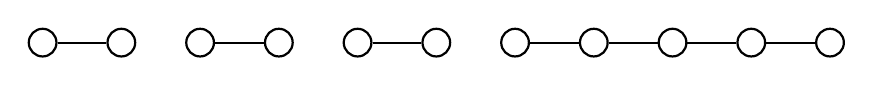
\begin{tikzpicture}[auto, thick]
\tikzstyle{vertex}=[draw,circle,text=violet,minimum width=10pt]
  \foreach \place/\name in {{(0,0)/a},
                            {(1,0)/b},
                            {(2,0)/c},
                            {(3,0)/d},
                            {(4,0)/e},
                            {(5,0)/f},
                            {(6,0)/g},
                            {(7,0)/h},
                            {(8,0)/i},
                            {(9,0)/j},
                            {(10,0)/k}}
    \node[vertex] (\name) at \place {};
  \foreach \source/\dest in {a/b,c/d,e/f,g/h,h/i,i/j,j/k}
      \path (\source) edge (\dest);
\end{tikzpicture} \vspace*{2.5ex}
    \caption{A foolproof scheme for $(\pa,\pb)=(3,8)$}
\end{figure}

\begin{figure}[!htb]
   \centering
    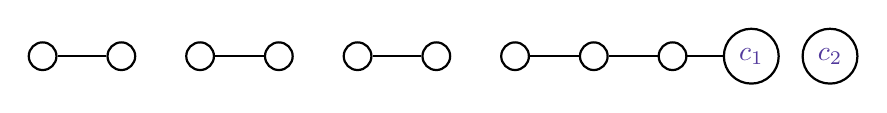
\begin{tikzpicture}[auto, thick]
\tikzstyle{vertex}=[draw,circle,text=violet,minimum width=10pt]
  \foreach \place/\name in {{(0,0)/a},
                            {(1,0)/b},
                            {(2,0)/c},
                            {(3,0)/d},
                            {(4,0)/e},
                            {(5,0)/f},
                            {(6,0)/g},
                            {(7,0)/h},
                            {(8,0)/i}}
    \node[vertex] (\name) at \place {};
  \node[vertex] (j) at (9,0) {$c_1$};
  \node[vertex] (k) at (10,0) {$c_2$};
  \foreach \source/\dest in {a/b,c/d,e/f,g/h,h/i,i/j}
      \path (\source) edge (\dest);
\end{tikzpicture} \vspace*{2.5ex}
    \caption{An $\IS^{+-}$ for $(\pa,\pb)=(3,8)$. If there is an unbalance edge, we infer the fake and real coin of the pair. If edges are all balance, we can infer the coin $c_1$ is real and the coin $c_2$ is fake.}
\end{figure}

Before discussing how to find an $\IS^{+-}$, we observe the range of $\tau^{+-}(a,b)$. Since $\tau(\pa,\pb)$ is sufficient to infer a fake coin and a real coin. 

\[
\tau^{+-} \leq \tau
\]

Through we cound infer a fake coin and a real coin, add this edge into the $\OIS^{+-}$, it's foolproof.

\[
\tau \leq \tau^{+-}+1
\]

Combine the inequations

\[
\tau-1 \leq \tau^{+-} \leq \tau
\]


Before solving $\IS^{+-}$, we observe how this works.

If \textbf{Condition 1.} happens then the solution works.
If \textbf{Condition 2.} happens, we infer a fake coin and a real coin. This pair is not in the $\IS^{+-}$. Adding this pair(edge) into the $\IS^{+-}$, the new graph is foolproof.

\begin{lemma}
Any inferable$^{+-}$ scheme is either a foolproof scheme or a foolproof scheme with an edge removed.
\end{lemma}

\begin{theorem}
Any optimal inferable$^{+-}$ scheme is either a optimal foolproof scheme or an optimal foolproof scheme with an edge removed.
\end{theorem}

Unlike infering a real-fake pair, removing an arbitrary edge from a $\OFS$ may not work.
We enumerate the edge removed for each $\OFS$ then check whether it's inferable$^{+-}$. 
Checking a scheme's inferability$^{+-}$ is similar to checking its inferability$^+$. Condition 1 is simple and the scheme to ganrantee Condition 2 don't happen is $\FS$. We shall focus on Condition 2. If Condition 2 happen can we infer a $+-$? To explain more, we return to the case Figure 4, the reason Figure 4 works is from lemma \ref{lma:inferable}. Because removing $c_1$'s component, the multiset [2,2,2,1] avoids $\pb$
\section{Open questions}
\subsection{Cycle happens earlier}
    As in theorem 4.3 and 4.4, we proved $\rho(\pa,\pb)$ would be in cycle for $\pb>d(d+1)(\pa-1)+(\pa-(\pa\mod d)$. But observing $\rho$table in Results 3.2, $\rho$ seems to get in cycle earlier. After computer comfirmation, we got results bellow.
    
\begin{tabular}{lll}
 $\pa$  & $\pb$: $\rho(\pa,\pb)$ start to cycle by theorem & $\pb$: $\rho(\pa,\pb)$ start to cycle by computer comfirmation \\
\hline
 1  & 1                                     & 1                                                   \\
 2  & 13                                    & 1                                                   \\
 3  & 15                                    & 5                                                   \\
 4  & 40                                    & 10                                                  \\
 5  & 29                                    & 9                                                   \\
 6  & 105                                   & 29                                                  \\
 7  & 43                                    & 13                                                  \\
 8  & 91                                    & 22                                                  \\
 9  & 57                                    & 17                                                  \\
 10 & 118                                   & 28                                                  \\
\hline
\end{tabular}

    Since the algorithm cost exponential time, we could only comfirm this in small case.
    
    But if it get in cycle earlier in general case, we can use a better(smaller) $K$ algorithm 4.1 and run faster.
\subsection{Avoidance integer partition}
    As in algorithm 3.1,4.1, to find an optimal solution require enumerating partitions of $\pa+\pb$ avoiding $\pa$. In the algorithms, we enumerating all partitions of $\pa+\pb$ and check if it avoids $\pa$. So the time complexity is analyzed as the (number of partitions) times checking avoidance. If exist a way to enumerate avoidance and bound it tighter, the time complexity would be better.

%!TEX root = total.tex

\bibliographystyle{plain}
\begin{thebibliography}{99}
\bibitem{Gro45}
Howard D.~Grossman.
The Twelve-Coin Problem, 
{\em Scripta Mathematica} XI, pages 360--361, 1945. 

\bibitem{GuyNow95}
Richard K.~Guy and Richard J.~Nowakowski.  
Coin-Weighing Problems, 
{\em The American Mathematical Monthly}, 102(2):164--167, 1995.

\bibitem{HalHun95}
Lorenz Halbeisen and Norbert Hungerb\"{u}hler. 
The General Counterfeit Coin Problem, 
{\em Discrete Mathematics},  147(1--3):139--150, 1995. 
\end{thebibliography}

\end{document}